% --- Deckblatt ---
\thispagestyle{empty} % Keine Kopf- und Fußzeile auf dem Deckblatt
%\sffamily % Serifenlose Schriftart (optional)

% --- Bild: Klein und zentriert am Anfang des Titels ---
\begin{picture}(0,0)(140, 253)
    
\includegraphics[width=0.7\linewidth]{Pictures/Deckblatt/MCI_forum_grau20.png}
\end{picture}

% --- Bild: Größer und zentriert in der Mitte der oberen Hälfte (optional) ---
%\begin{picture}(0,0)(35,400)
%    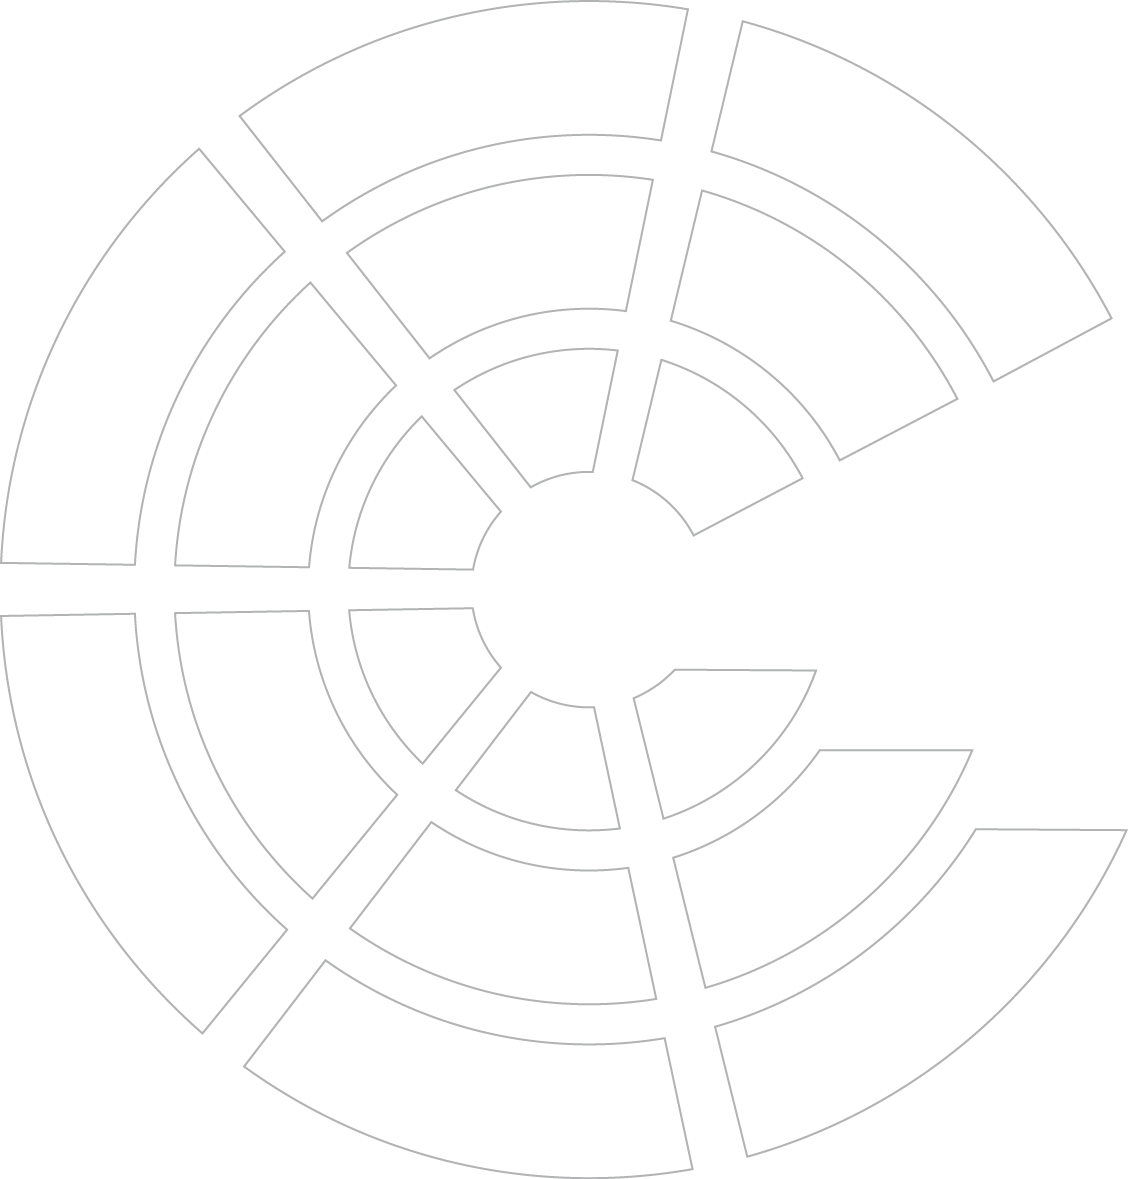
\includegraphics[width=1.2\linewidth]{Pictures/Deckblatt/MCI_forum_outline_grau40.png}
%\end{picture}

{\bfseries % Fett formatierter Bereich beginnt

\vspace*{3cm}

% --- Titel: Laborbericht ---
\def\thesis{Laserablenksystem} % Makro für das Wort "Laborbericht"
\textcolor{black}{\rmfamily\bfseries\huge\thesis} % Serifenschrift, fett und groß

\vspace*{0.5cm}

% --- Titelzeile mit Laborinformationen ---
\textbf{\labtitle{ }(\labcode)}% Titel und Code des Labors

\labname % Name des Labors

%\labnum, \labdate % Nummer und Datum der Laborübung (optional)

\vspace*{14cm} % Abstand zur unteren Hälfte des Deckblatts

\begin{footnotesize}

% --- Studieninformationen ---
\textcolor{gray}{\study} % Studienrichtung
\textcolor{gray}{\studygroup} % Studiengruppe

% --- Semesterinformationen ---
\def\termname{Semester} % Makro für "Semester"
\textcolor{gray}{\term{ }\termname} % Semesterangabe

% --- Lehrveranstaltungsleiter ---
\def\lecturername{Lehrveranstaltungsleiter} % Makro für "Lehrveranstaltungsleiter"
\textcolor{gray}{\lecturername: \lecturer} % Name des Dozenten

% --- Jahrgangsinformation ---
\def\groupname{Jahrgang} % Makro für "Jahrgang"
\textcolor{gray}{\groupname: \group} % Jahrgang

% --- Verfasserinformationen ---
\def\authorname{Verfasser} % Makro für "Verfasser"
\textcolor{gray}{\authorname: \student} % Autorenliste

% --- Mitwirkendeinformationen ---
%\def\contributorname{Mitwirkender} % Makro für "Mitwirkende"
%\textcolor{gray}{\contributorname: \contributor} % Mitwirkendenliste

% --- Datum ---
\textcolor{gray}{\today} % Heutiges Datum in Grau
    
\end{footnotesize}

\newpage % Neue Seite nach dem Deckblatt
} % Ende des fett formatierten Bereichs